\subsection{Fast-forwarding}
\label{subsec:eval-ff}

In this section,
  we evaluate our new \ff algorithm (\autoref{sec:lift})
  in two new domains to learn rewrite rules
  that other state-of-the-art tools
  do not support.
We also show that synthesized rules from \enumo
  can be easily integrated with
  existing \eqsat-based synthesis tools.

\begin{table}[h]
\resizebox{\textwidth}{!}{%
\begin{tabular}{lllccc}
Domain      & \enumo LOC  & \# \enumo (Time)  & \# \herbie  & \enumo $\rightarrow$ \herbie (Time) & \herbie $\rightarrow$ \enumo (Time)  \\ \cline{1-6}
  Exponential &  186  & 40 (3.58)    & 82 &  39.0\% (1.03), 43.9\% (1.25)   & 100\% (0.24), 100\% (0.01) \\
  Rational    &   82  & 129 (276.16) & 87 &  70.1\% (54.77), 73.6\% (55.19) &  -, -\\
  Trigonometric  &  160  & 56 (631.94)  & 45 &  33.3\% (4.20), 35.6\% (7.36) & 46.4\% (0.84), 46.4\% (2.27)\\
\end{tabular}%
}
  \caption{
  Derivability comparison between rules from \enumo and \herbie.
  As in \autoref{table:oopsla},
    $R_1 ~ \rightarrow ~ R_2$ indicates using
    $R_1$ to derive $R_2$ rules.
  For Exponential and Trigonometric, we include the trusted arithmetic
    rules defined below (\C{RAT}, and \C{R} without its division
    rules) when computing the derivability.
  We report both \lhs and \lhsandrhs derivability
    (in that order), separated by commas. The numbers in parentheses
    are times in seconds.
 ``-'' indicates that the derivability test
    could not be completed due to \herbie's
    unsound rules (\autoref{para:herbie}).
  We integrate these rules for
    end-to-end runs of \herbie~\citep{herbie} and
    Megalibm~\citep{megalibm} (\autoref{subsubsec:numbers}).}
\label{table:herbie}
\end{table}

\subsubsection{Numeric domain}
\label{subsubsec:numbers}

We used the fast-forwarding algorithm together with
  guided enumeration to infer rewrite rules
  for the domain of transcendental functions.
To evaluate the quality of the rulesets,
  we integrated the rules into two existing
  rewrite-rule-based synthesis tools,
  \herbie~\citep{herbie} and
  Megalibm~\citep{megalibm}.

\paragraph*{Trigonometric and exponential representation.}
\label{eval:trig-rep}

Recall that sine and cosine have representations
  in terms of the complex exponential $\cis(x)$
  (\autoref{subsec:ffoverview}).
The trusted rules for the Trigonometric domain fall into three groups, which we refer
  to throughout the evaluation:
\begin{itemize}
  \item \C{R}: 57 automatically generated arithmetic rules,
    including 13 rules involving division that are sound only when their divisors are nonzero\footnote{
      In our \enumo programs for this domain, we are careful to exclude undefined terms from the \egraph,
      so the potentially unsound rules are harmless. Herbie uses unsound rules in its \eqsat
      runs, but with extra checks to detect unsound merges and recover from them.
    }.
  \item \C{C}: 15 handwritten rules about the complex exponential, including rules like
  $\cis(a + b) \leftrightsquigarrow \cis(a) \cdot \cis(b)$,
  $\cis(0) \leftrightsquigarrow 1$, and $i \cdot i \leftrightsquigarrow -1$.
  \item \C{E}: 18 \textit{exploratory} rules (\autoref{sec:lift}), which
    give the definitions of $\sin$, $\cos$, and $\tan$ in terms of $\cis$, $i$, and $\pi$.
\end{itemize}

Similarly, the logarithmic, power, square root,
  and cube root functions are all defined in terms of $e^x$,
  the real exponential function:
  $e^{\log(x)} \leftrightsquigarrow x$,
  $a^b \leftrightsquigarrow e^{b \cdot \log(a)}$,
  $\sqrt{a} \leftrightsquigarrow e^{1/2 \cdot \log(a)}$, and
  $\sqrt[3]{a} \leftrightsquigarrow e^{1/3 \cdot \log(a)}$.
In the exponential domain, we have two trusted rulesets:
\begin{itemize}
  \item \C{RAT}: 141 automatically generated arithmetic rules
  \item \C{EXP}: 13 handwritten rules involving the real exponential function,
    which include rules that define
    $\log$, powers, and roots in terms of $e^x$,
  to bootstrap fast-forwarding.
\end{itemize}
For both the exponential and trigonometric domains,
  the set of known arithmetic rules can be produced by
  \enumo~via methods described in previous sections.

\paragraph*{\herbie.}

\herbie~\citep{herbie} is a widely used, open-source tool
  for improving the accuracy of floating-point expressions.
Given a mathematical expression over real numbers,
  it synthesizes a more accurate
  floating-point implementation
  using a variety of techniques
  including equality saturation.
\herbie's equality saturation-based optimization pass
  uses a set of 358 expert-written rewrite rules
  to explore many programs
  that are equivalent over the reals,
  keeping only those that have
  lower floating-point error.
\herbie's rewrite rules include many algebraic identities
  about rational arithmetic, trigonometry, and exponents.

\paragraph*{Results.}
\label{para:herbie}
\begin{figure}
  \begin{subfigure}[t]{0.49\linewidth}
    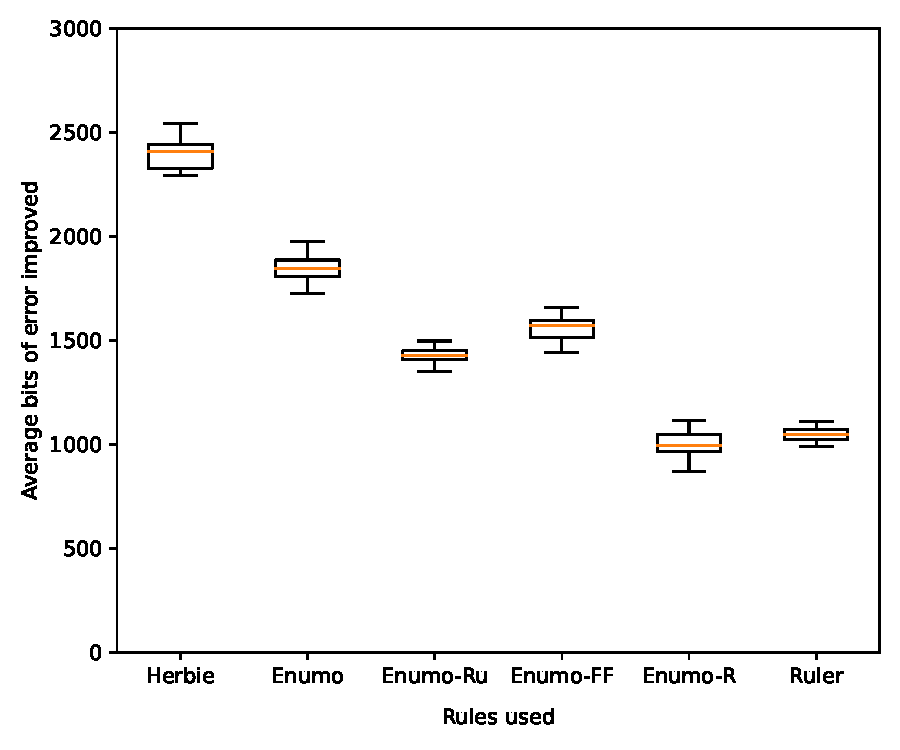
\includegraphics[width=\linewidth]{fig/herbie/err-improve.pdf}
  \end{subfigure}
  \hfill
  \begin{subfigure}[t]{0.49\linewidth}
    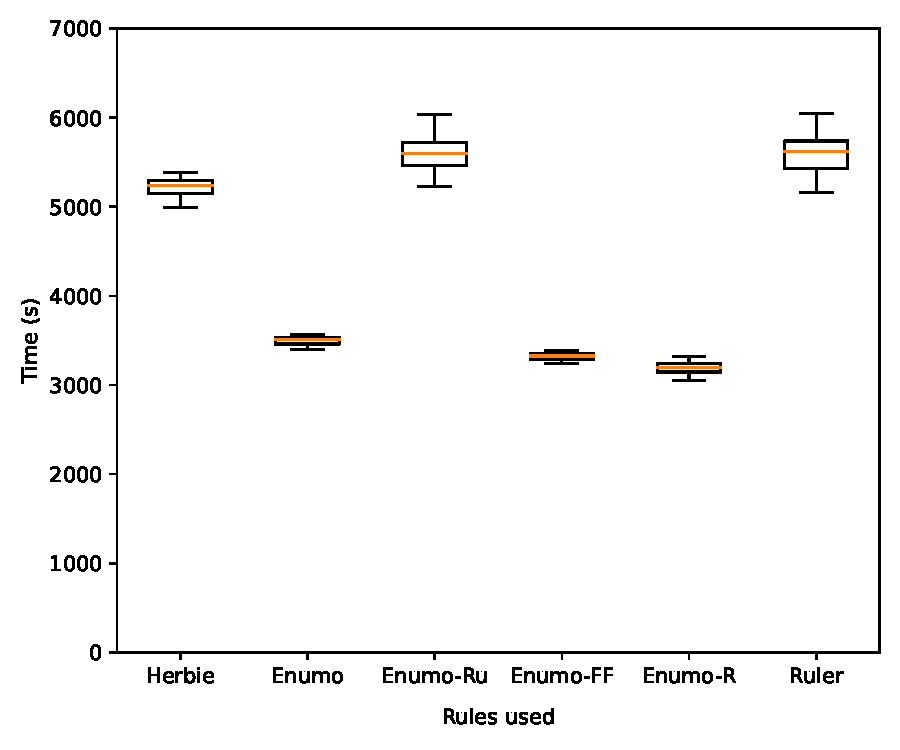
\includegraphics[width=\linewidth]{fig/herbie/time.pdf}
  \end{subfigure}
  \caption{
    Comparison of different rules on \herbie's
      end-to-end performance for six different configurations:
      \herbie's default rules (\texttt{Herbie}),
      \enumo's rules (\texttt{\enumo}),
      \enumo's rules with its rational rules replaced by \ruler's rational rules (\texttt{\enumo-Ru}),
      \enumo's rules without fast-forwarded rules (\texttt{\enumo-FF}),
      \enumo's rational rules (\texttt{\enumo-R}),
      and \ruler's rules (\texttt{\ruler}).
    The two plots show
      (left) \herbie's metric for measuring accuracy (higher is better); and
      (right) \herbie's running time (lower is better).
    Each boxplot represents the results from 30 seeds,
     where each data point is obtained by summing the values
     (average error, time) over the 170 benchmarks that
     finish within the time limit.
    \enumo's rules allow \herbie to improve error
      significantly more than \ruler's rules.
  }%
  \label{fig:herbie-res}
\end{figure}

First, we wrote \enumo programs to synthesize boolean,
  rational, trigonometric (fast-forwarded),
  and exponential (fast-forwarded) rules for \herbie.
The summary of these results is in \autoref{table:herbie}.
Note that \enumo's rules derive only about a third of
  \herbie's trigonometric ruleset:
  \herbie's handwritten rules include forms beyond
  the scope of our workloads and, as discussed below,
  some unsound rules that no sound ruleset can derive.
Then, based on suggestions from \herbie's developers,
  we filtered the \herbie benchmark suite to 176
  representative benchmarks, taken from a variety of domains,
  including graphics, mathematics, and numerical analysis.
In addition, we disabled polynomial approximation to
  isolate the effects of \eqsat within \herbie.
We ran \herbie on the benchmarks under six different configurations:
\begin{itemize}
  \item \foottt{\herbie}: \herbie's default configuration.
  \item \foottt{\enumo}: \enumo's rules, including boolean, rational, trigonometric, and exponential.
  \item \foottt{\enumo-Ru}: \enumo's rules with its rational rules replaced by \ruler's rational rules. This includes \enumo's boolean, trigonometric, and exponential rules, and also \ruler's rational rules.
  \item \foottt{\enumo-FF}: \enumo's rules without fast-forwarded rules.
  \item \foottt{\enumo-R}: \enumo's rules, including only
  boolean and rational rules.
  \item \foottt{Ruler}: We compare against \ruler's rules~\citep{ruler}
    for the rational and boolean domains.
    \ruler does not support the trigonometric and exponential domains.
\end{itemize}

We used the default node limit of 8000 nodes
  in \herbie's underlying \eqsat engine,
  i.e., upon hitting the limit,
  the engine stops applying the simplification rules.
On 6 benchmarks, \herbie does not finish
  within 300 seconds; we discard these.
For all six configurations,
  we ran \herbie on 30 seeds.

\autoref{fig:herbie-res} shows the results of running
  \herbie with one boxplot for each ruleset configuration.
The left plot
  shows the improvement in accuracy achieved by \herbie,
  measured in \herbie's ``bits of error'' metric:
  the number of ``incorrect'' bits
  in the binary representation of the floating-point
  result against a high-precision oracle
  (higher improvement is better).
The right plot shows the average running time of \herbie;
  \enumo's rules consistently yield faster runs
  than \ruler's rules.
\herbie's handwritten ruleset (\herbie) finds the
  most accurate programs, followed by \enumo's rules.
This experiment offers two key takeaways:
  (1) \ff is valuable in practice, and (2) \ff and
  guided search combined lead to better rulesets than
  exhaustive synthesis alone.

Disabling trigonometric and exponential rules (\texttt{\enumo-FF}),
  \emph{but leaving the rules needed to bootstrap fast-forwarding},
  results in a significant drop in accuracy,
  demonstrating that fast-forwarding is necessary in
  the face of resource limits.
By definition, the rulesets from both \texttt{\enumo} and \texttt{\enumo-FF} have equal proving power,
  but \autoref{fig:herbie-res} demonstrates
  a significant advantage for \texttt{\enumo} over \texttt{\enumo-FF} in practice.
Using only the rational rules (\texttt{\enumo-R}) also results in lower accuracy,
  showing that trigonometric and exponential rewrite rules are important for \herbie.

To our surprise,
  Ruler's rational rules (\texttt{\ruler}) outperformed
  those from \enumo (\texttt{\enumo-R}).
However, we show that when combined with the rest of
  \enumo's ruleset (\texttt{\enumo}), \enumo finds more accurate programs
  faster than \ruler.
Replacing \enumo's rational rules with \ruler's (\texttt{\enumo-Ru})
  results in a significantly worse ruleset.
The reason is that the combination of \enumo's rational ruleset
  and \enumo's trigonometric and exponential rules allows \herbie
  to fix a wider range of floating-point errors.
We suspect that \enumo's rational rules (\texttt{\enumo-R}) explore a larger
  space than \ruler's (causing \herbie to exceed resource limits faster)
  without any benefit, leading to a slight accuracy loss compared to
  \ruler's rational rules.

An example of where rules from \enumo excel over rules from \ruler
  is \herbie's ``2cos''%
  \footnote{\url{https://github.com/herbie-fp/herbie/blob/d35c6a3cc7ab/bench/hamming/trigonometry.fpcore}}
  benchmark, $\cos(x + \varepsilon) - \cos x$,
  which suffers from error when $\varepsilon$ is relatively small.
With \enumo's ruleset,
  \herbie~uses the essential rewrite
  \C{(cos (+ b a)) \rewritesto ~} \\
  \C{(- (* (cos b) (cos a)) (* (sin b) (sin a)))}
  to decompose $\cos(x + \varepsilon)$, and then
  eliminates cancellation using associative rules.
The full rewrite is
  $\cos(x + \varepsilon) - \cos x
  \rightsquigarrow
  \cos x \cdot (\cos\varepsilon + -1) + \sin x \cdot (-\sin\varepsilon)$.

However, \herbie still finds more accurate programs
  with its handwritten ruleset.
One significant reason for this difference is that
  \herbie often relies on unsound
  division, trigonometry, and exponentiation rules in order
  to eliminate sources of errors
  such as cancellation without checking if
  such transformations are correct for all arguments.
For example,
  for the benchmark ``2sin''%
  \footnote{\url{https://github.com/herbie-fp/herbie/blob/d35c6a3cc7ab/bench/hamming/trigonometry.fpcore}},
 \herbie rewrites
 $\sin \left(x + \varepsilon\right) - \sin x$ to
 $\cos x \cdot \sin \varepsilon + ({\sin \varepsilon}^{2} \cdot \sin x)/(-1 - \cos \varepsilon)$
 using a series of rewrites including the unsound
 factoring rule
 \C{(+ a b)} \rewritesto ~ \C{(/ (- (* a a) (* b b)) (- a b))},
 which is invalid when \C{a} equals \C{b}.
In contrast, \enumo generates a conditional
  factoring rule with the side condition $(- a b) \neq 0$.
Unfortunately, \herbie is not designed to leverage conditional rules.
With \enumo, however, we can instead reify the guard syntactically
  within the rewrite itself.
\herbie can directly apply such rules, e.g.,
  \C{(+ a b)}
  \rewritesto ~
  \C{(if (- a b)
         (/ (- (* a a) (* b b)) (- a b))
         (+ a b))},
relying on other rules to simplify the condition syntactically.
\herbie's use of unsound rules and its lack of support
  for conditional rules pose a significant challenge in
  closing the gap between its handwritten rules
  and \enumo's generated rules.

